\chapter{Results}

\section{Tire/road friction for different driving sessions}
\todo{Write something nice inledande shit!}

To eliminate minor disturbances the combined force for the two front tires are used when calculating the force from the different models, rather than splitting it up into two different computations. This means that only one friction coefficient will be approximated rather than one for the respective sides. It would be referable to be able to calculate the friction coefficient for both sides in order to detect a split-$ \mu $ situation, but the trade off with ahving a more stable friction estimation is prioritized.

Note that the plots for the tire forces in this section only include the values where the actual friction estimation is done. When the conditions mentioned in Section \ref{when_to_estimate} are not fulfilled, the tire force value is set to zero. 


\subsection{Winter tires on asphalt}
The algorithm that approximates the friction coefficient was run on the straight line acceleration run used in Section \ref{winter_tire} to acquire the tire model parameters. The combined forces from both tires can be seen with the respective force models in Figure \ref{force_mue_olika_acc}, subplot one. The corresponding friction coefficient can be seen in subplot two. 

\begin{figure}[h]
	\centering
	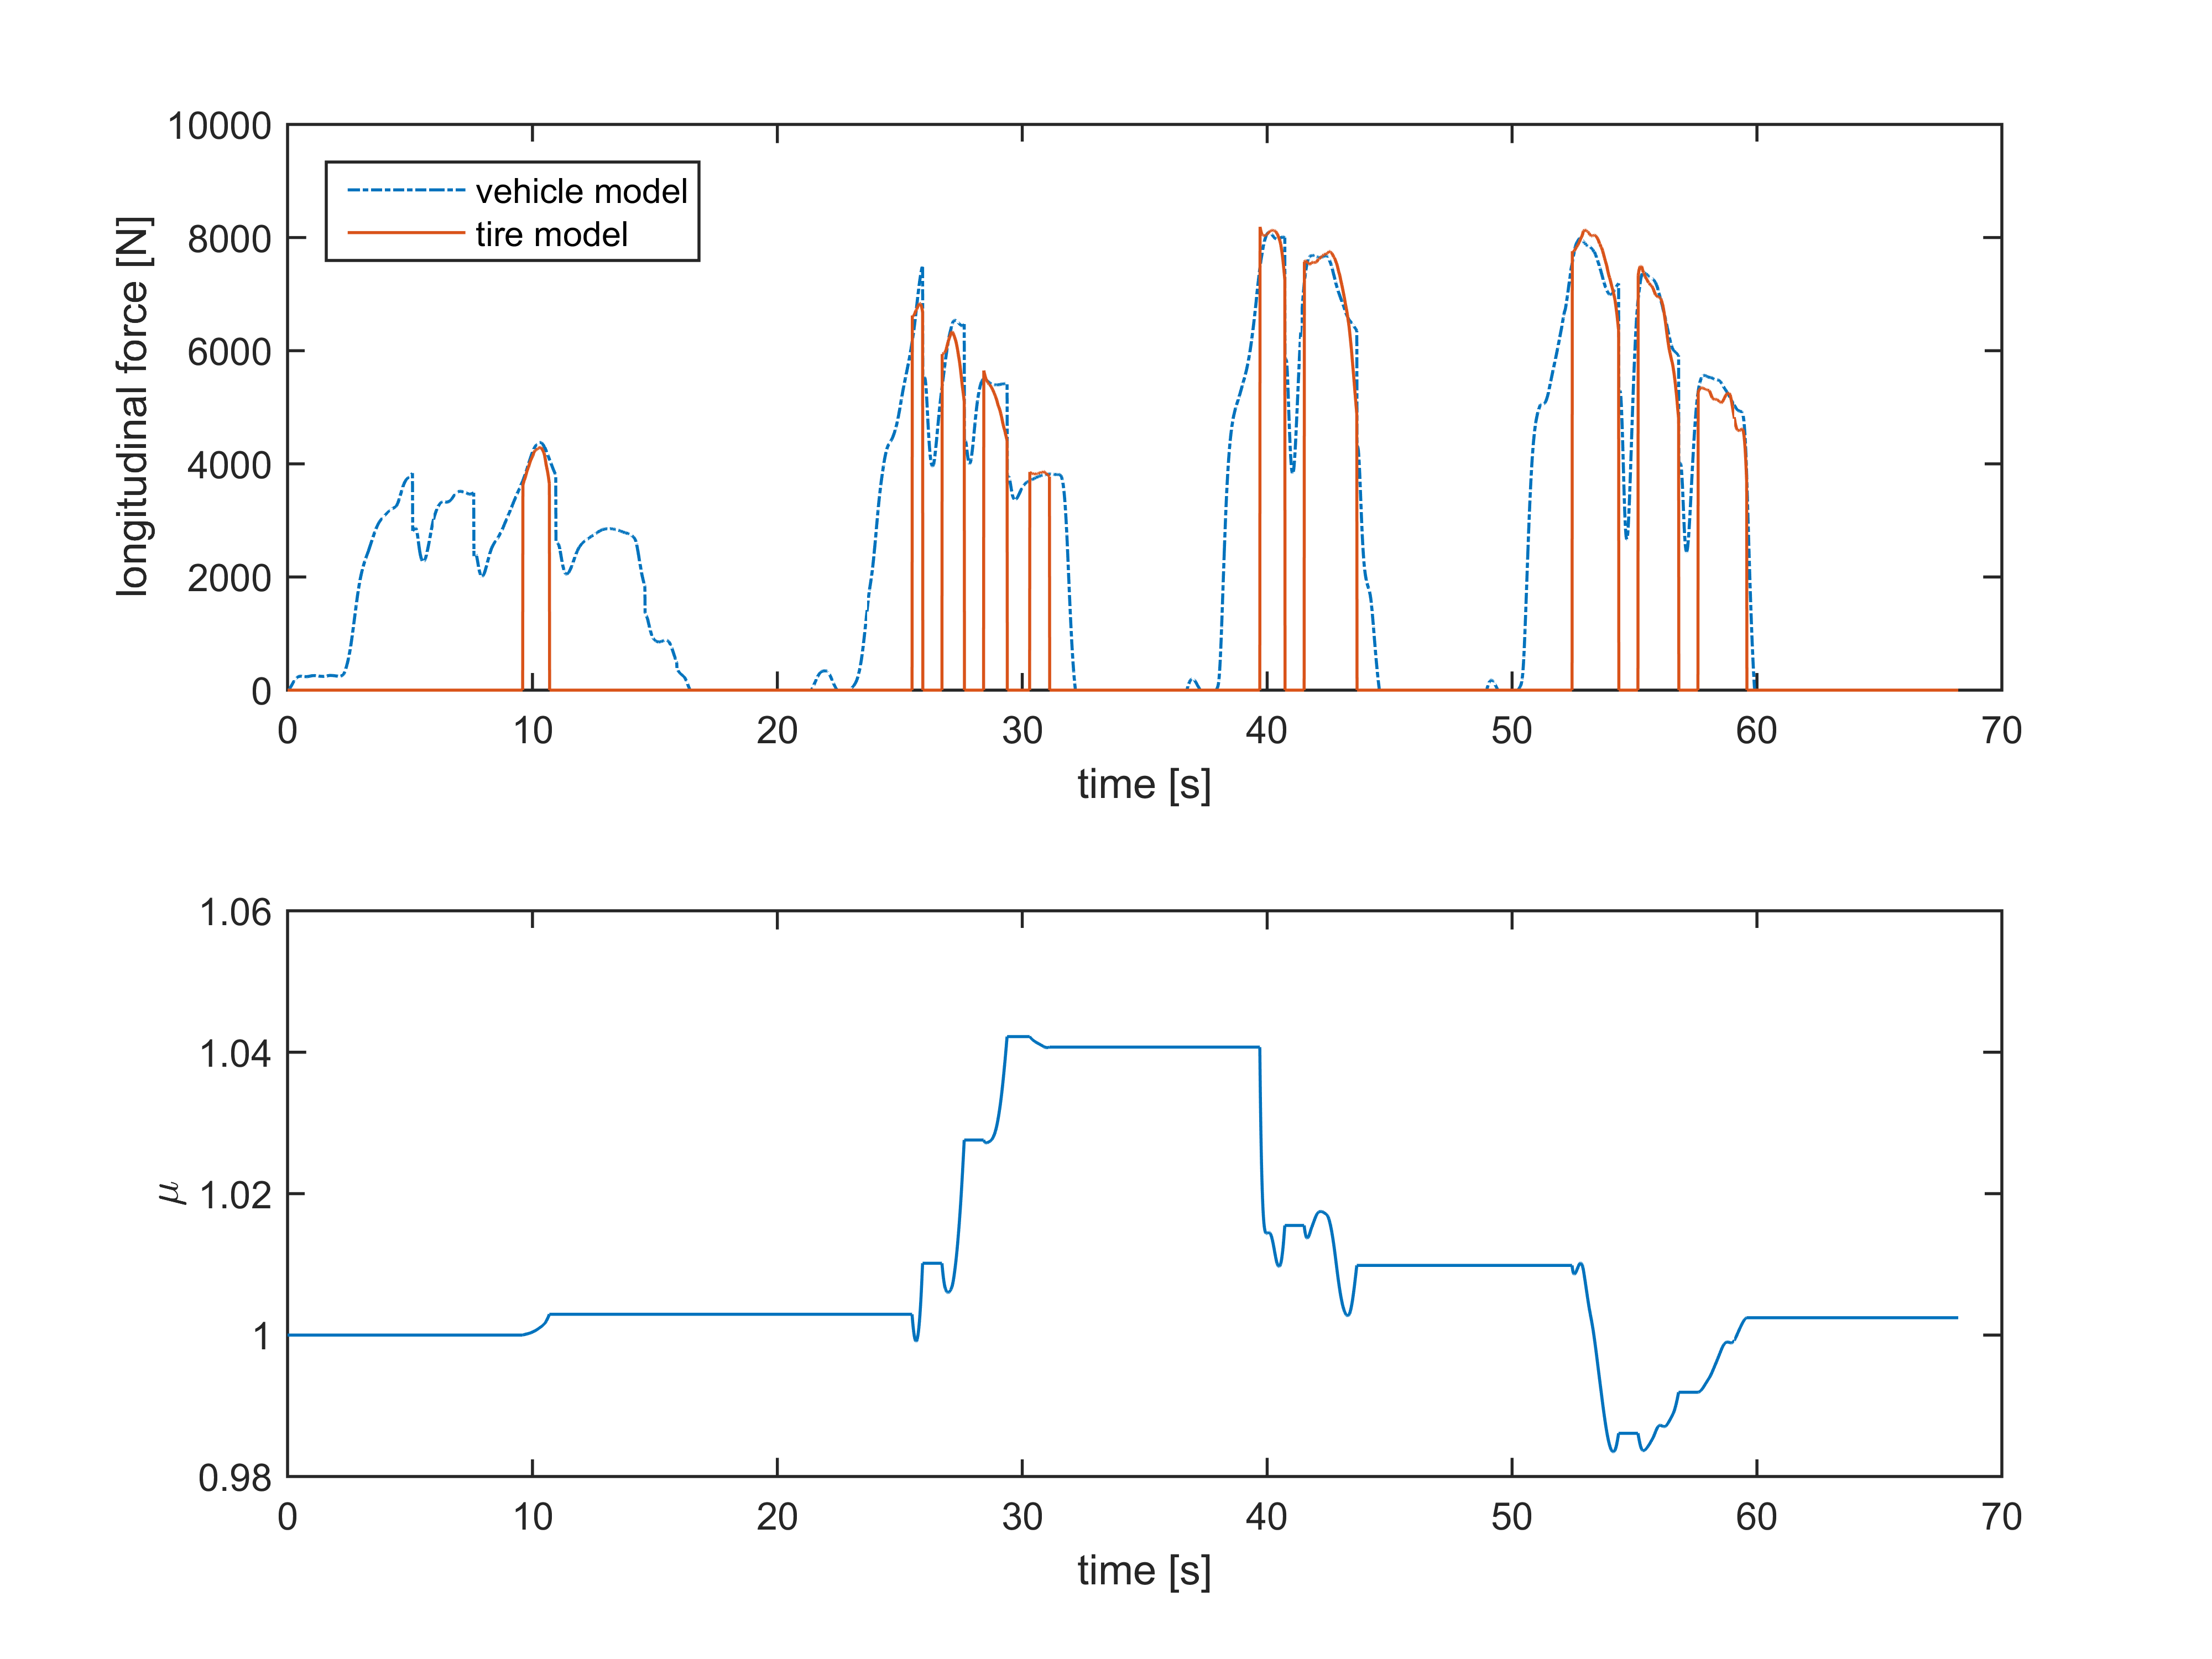
\includegraphics[width=1.0\textwidth]{Pictures/force_mue_olika_acc}
	\caption {Force from the tire and vehicle model and the approximated $ \mu $ for a straight line acceleration.}
	\label{force_mue_olika_acc}
\end{figure}

The friction estimation can seem to be jumpy at certain times, but the changes of frictional value are still quite small. The friction estimation stays around $ \mu = 1 $, which it evidently should due to the fact that the tire model parameters are fitted during this driving sequence.  

A more interesting test for the friction estimation algorithm is a driving sequence done as the fast track run. The same tires were used on a similar surface as in the previous driving sequence. The force from the two models and the friction estimation result can be see in Figure \ref{force_mue_race}. 

\begin{figure}[h]
	\centering
	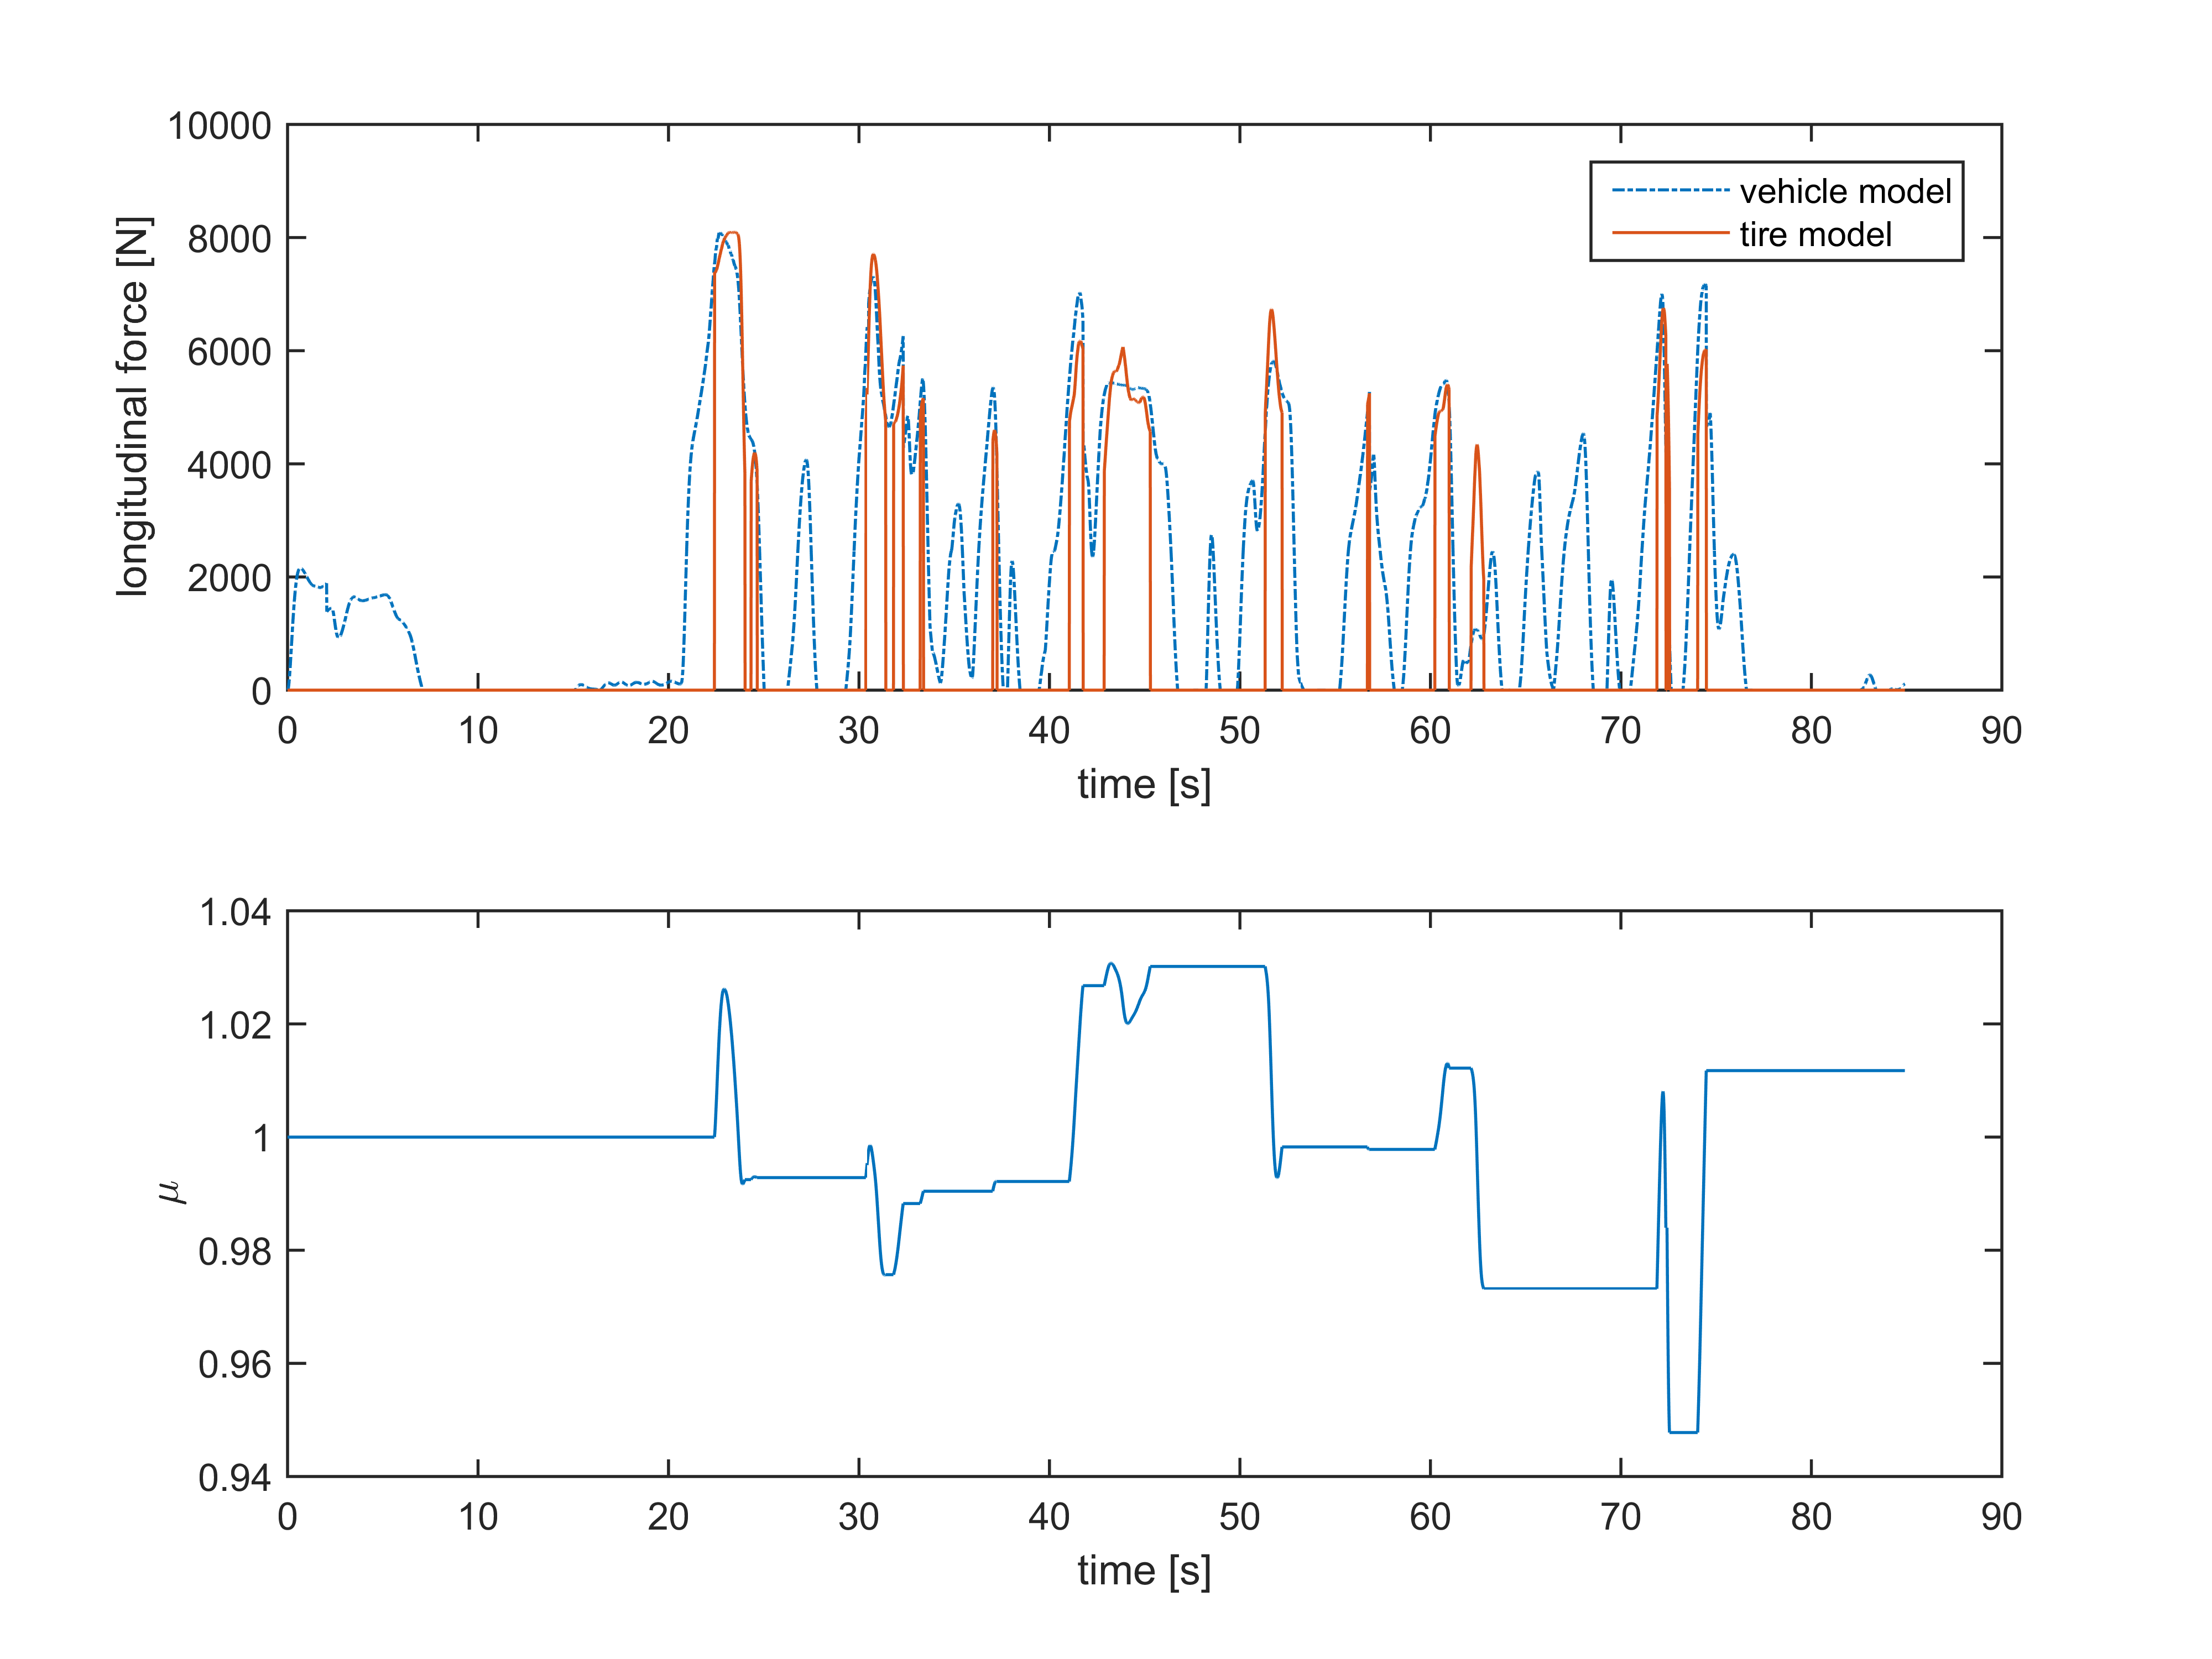
\includegraphics[width=1.0\textwidth]{Pictures/force_mue_race}
	\caption {Force from the tire and vehicle model and the approximated $ \mu $ for a fast track run.}
	\label{force_mue_race}
\end{figure}

The resulting friction coefficient is seen to vary around $ \mu = 1 $, similar to the straight line acceleration run. The force from the tire model is seen to be calculated quite rarely in the first subplot, meaning that the friction coefficient is only approximated during these moment. However, the resulting $ \mu $ for these moments are fairly steady around $ \mu = 1 $. 

\subsection{Winter tires on ice}
Being able to detect a surface with a low friction coefficient is probably the most important part of the friction estimation algorithm, due to the risk of an accident if too much torque is transferred to one of the driving axles. The resulting forces from the models and the approximated fricion coefficient can be seen in Figure \ref{force_mue_ice_normal}.

\begin{figure}[h]
	\centering
	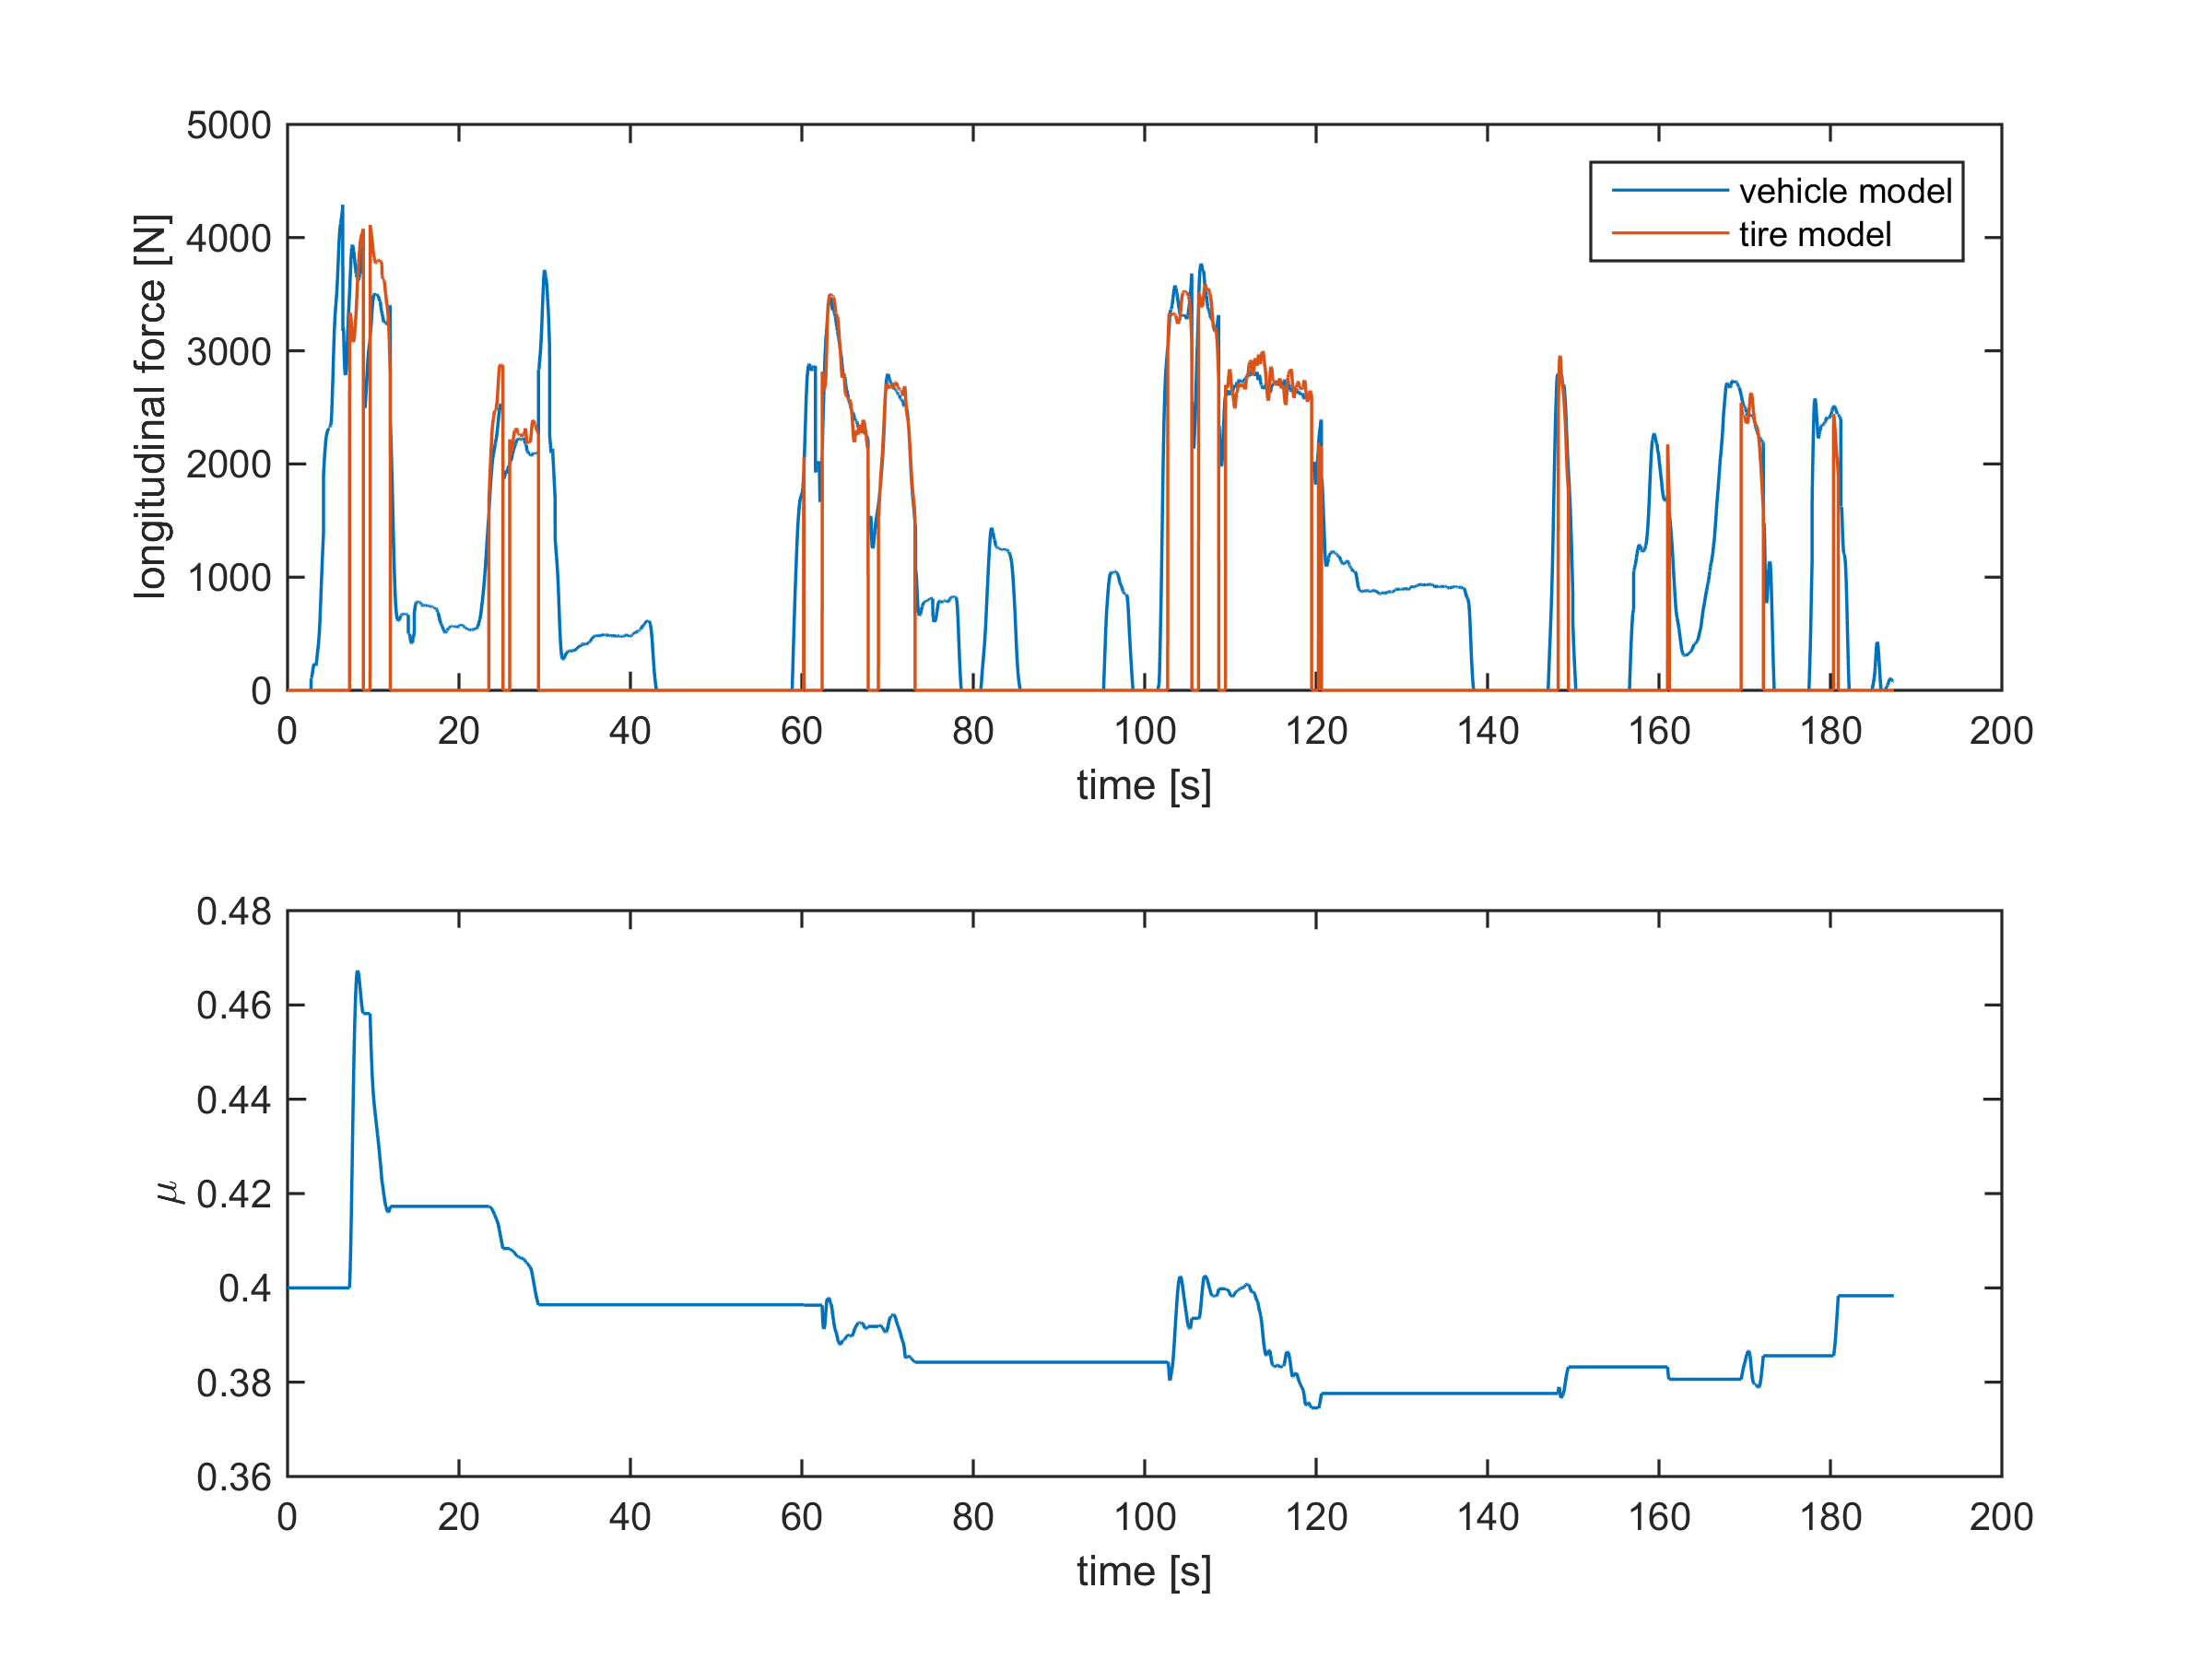
\includegraphics[width=1.0\textwidth]{Pictures/force_mue_ice_normal}
	\caption {Force from the tire and vehicle model and the approximated $ \mu $ for a fast track run.}
	\label{force_mue_ice_normal}
\end{figure}

The winter tire model parameter for low-$ \mu $ was fitted on this run. It is therefore no coincidence that the friction coefficient end up at around $ \mu = 0.4 $. It can be seen in the figure that the force calculated from the tires model varies with a higher frequency during the driving sequence on ice/snow compared to the previous sequences. Even though, the resulting friction coefficient is approximated fairly well around friction $ \mu = 0.4 $, except for a quite large differing $ \mu $ at the times $ \approx 7  - 12$ s.

\subsection{Winter tires on asphalt and ice combined}
The main goal for the work done in this report was to detect when low-$ \mu $ is present so that the torque transfer through the FXD can be limited. It is therefore essential to test the developed algorithm during a driving sequence that actually includes a changing $ \mu $, preferably from high-$ \mu $ to low-$ \mu $. It has not been possible to test this on a single run, for example on asphalt driving into a skid pad. In order to simulate this behavior, two different runs have been merged together, where the friction coefficient changes three times. The sequence merging was made at points where both sequences were accelerating or decelerates at the same velocity, in order to avoid unnecessary jumps. The merged result can be seen in Figure \ref{force_mue_comb2}. The approximated friction coefficient is seen to clearly change between the different driving sequences, meaning that the algorithm definitely manages to find that the grip between the tire and the road differs.
 
\begin{figure}[h]
	\centering
	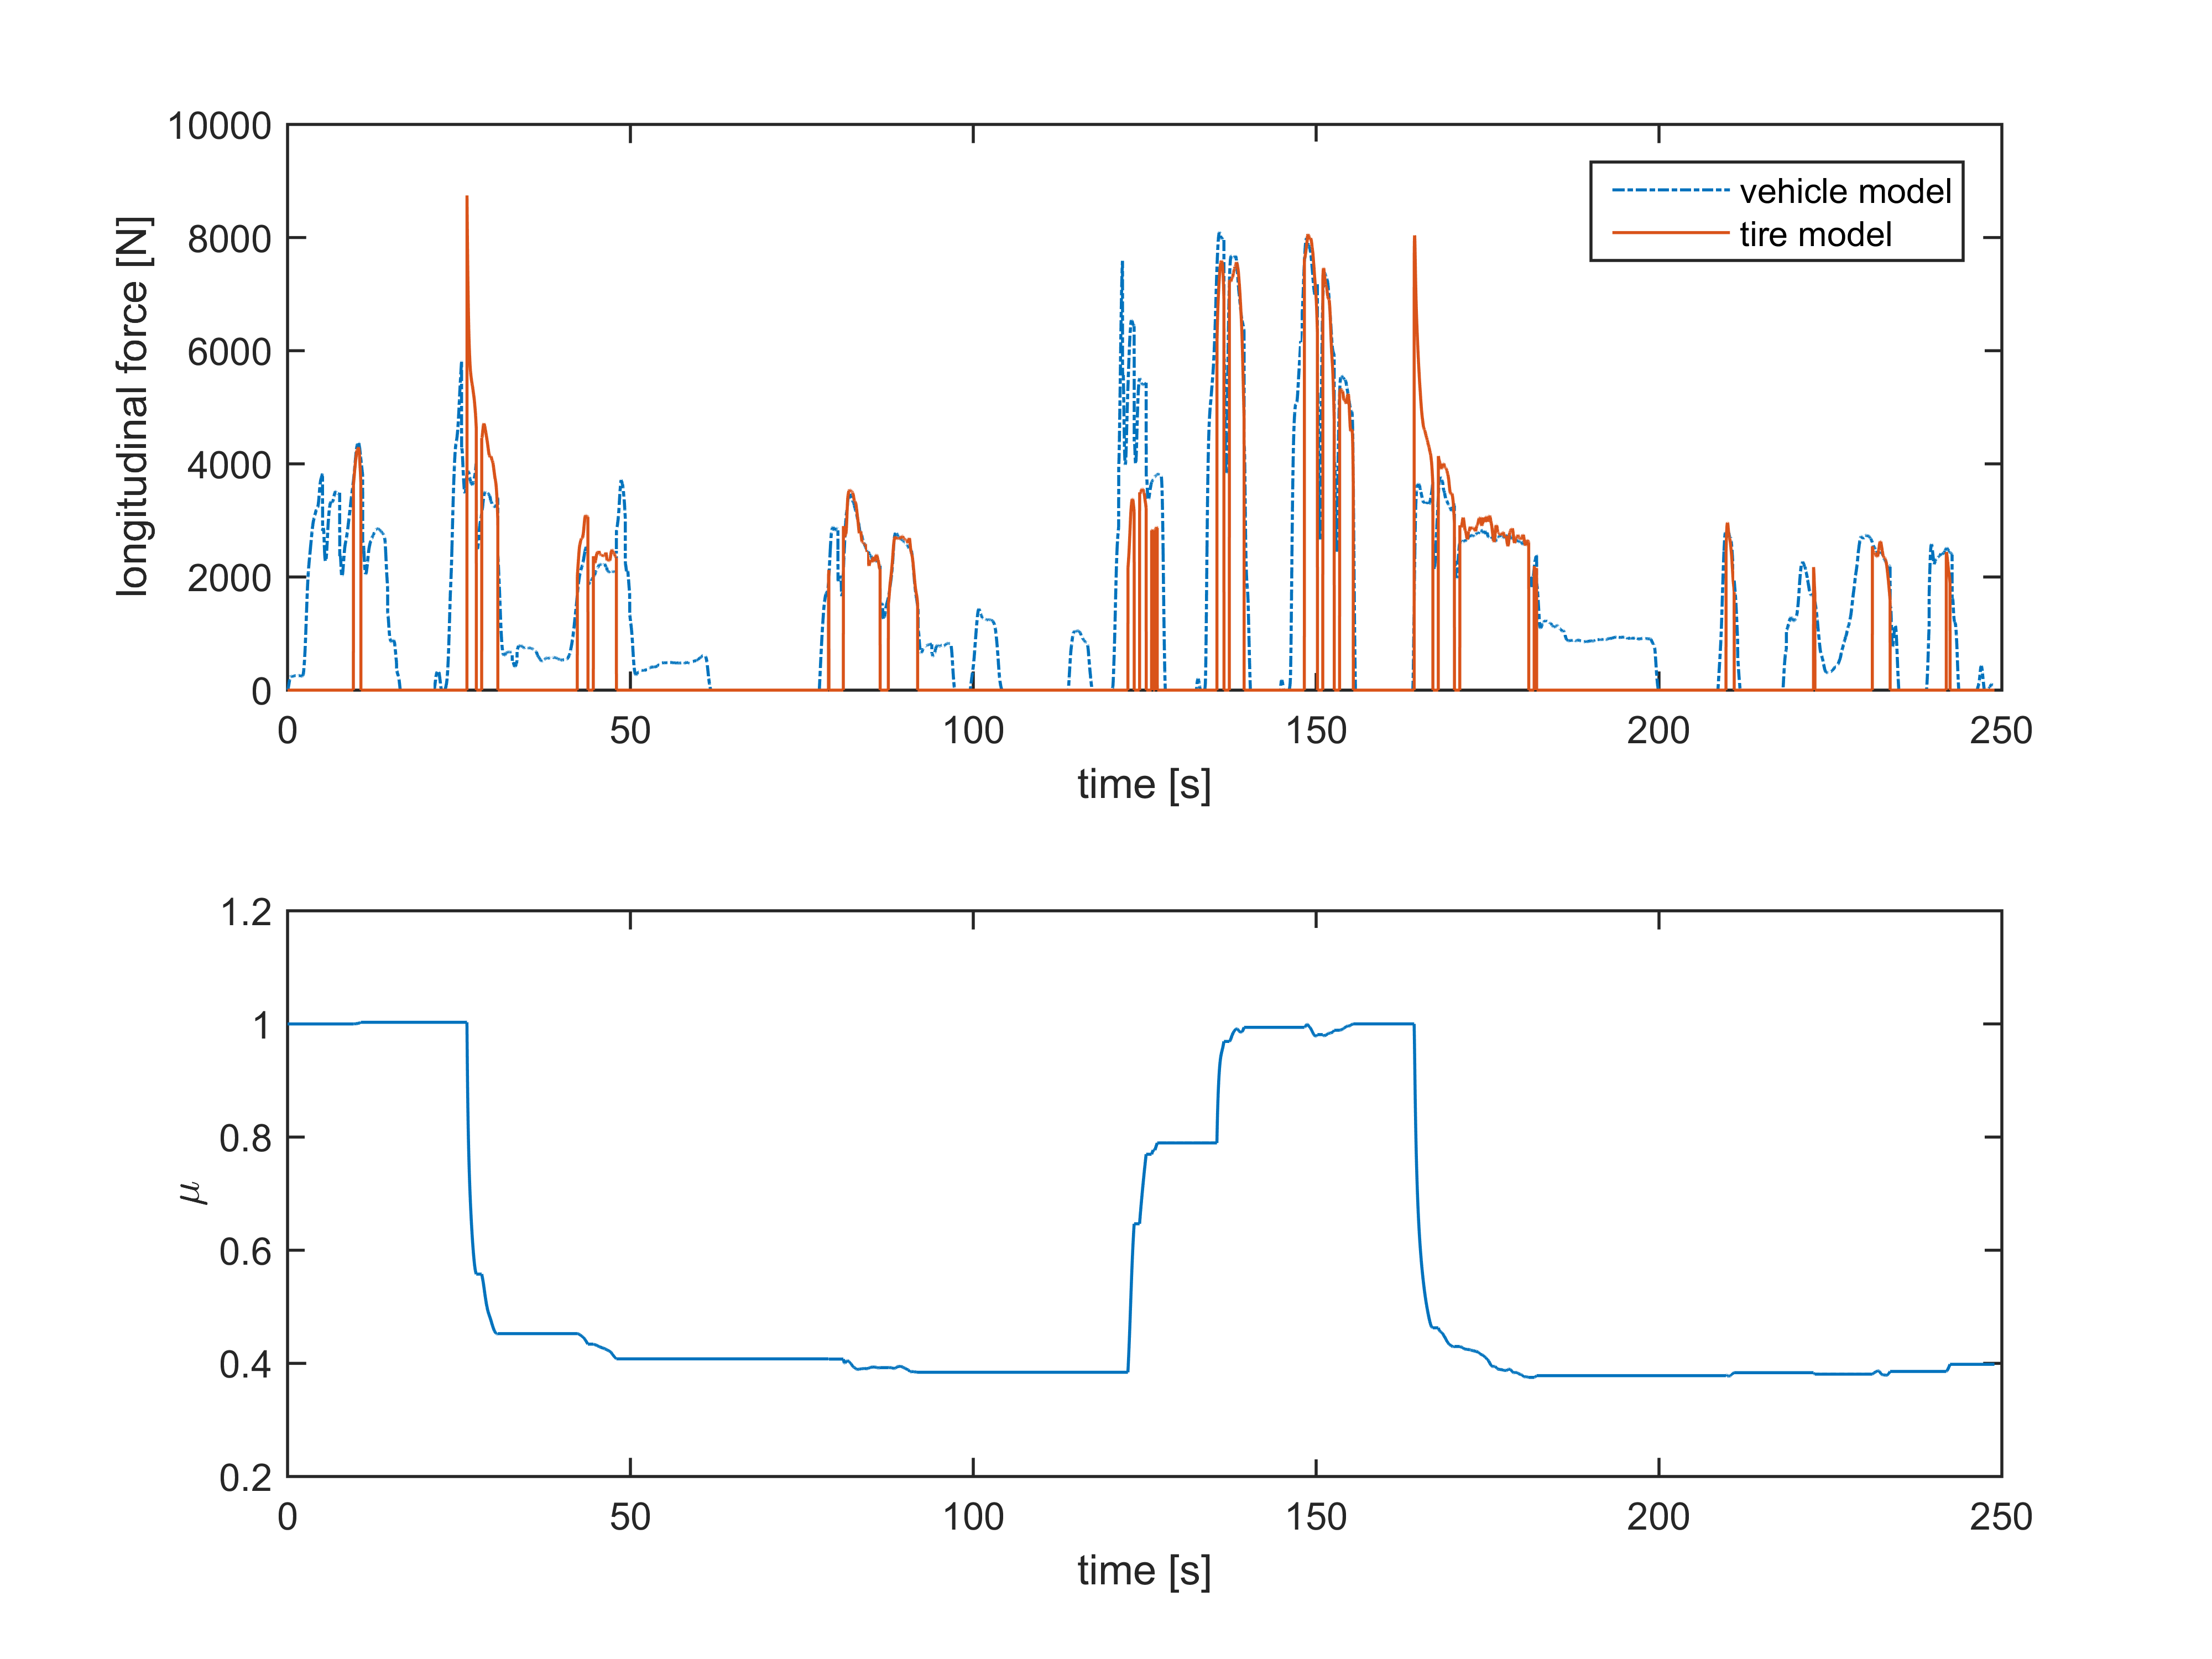
\includegraphics[width=1.0\textwidth]{Pictures/force_mue_comb2}
	\caption {Force from the tire and vehicle model and the approximated $ \mu $ for two different runs merged together.}
	\label{force_mue_comb2}
\end{figure}

Due to the limitations set concerning when the friction coefficient should be approximated, the algorithm's updated $ \mu $ may be delayed compared to the actual friction to the surface. However, when the algorithm is allowed to approximate, the new friction coefficient is approximated with good speed. In Figure \ref{force_mue_comb2_zoom}, the two forces and the friction coefficient can be seen when the result is zoomed in on a sudden drop of the friction coefficient. 

\begin{figure}[h]
	\centering
	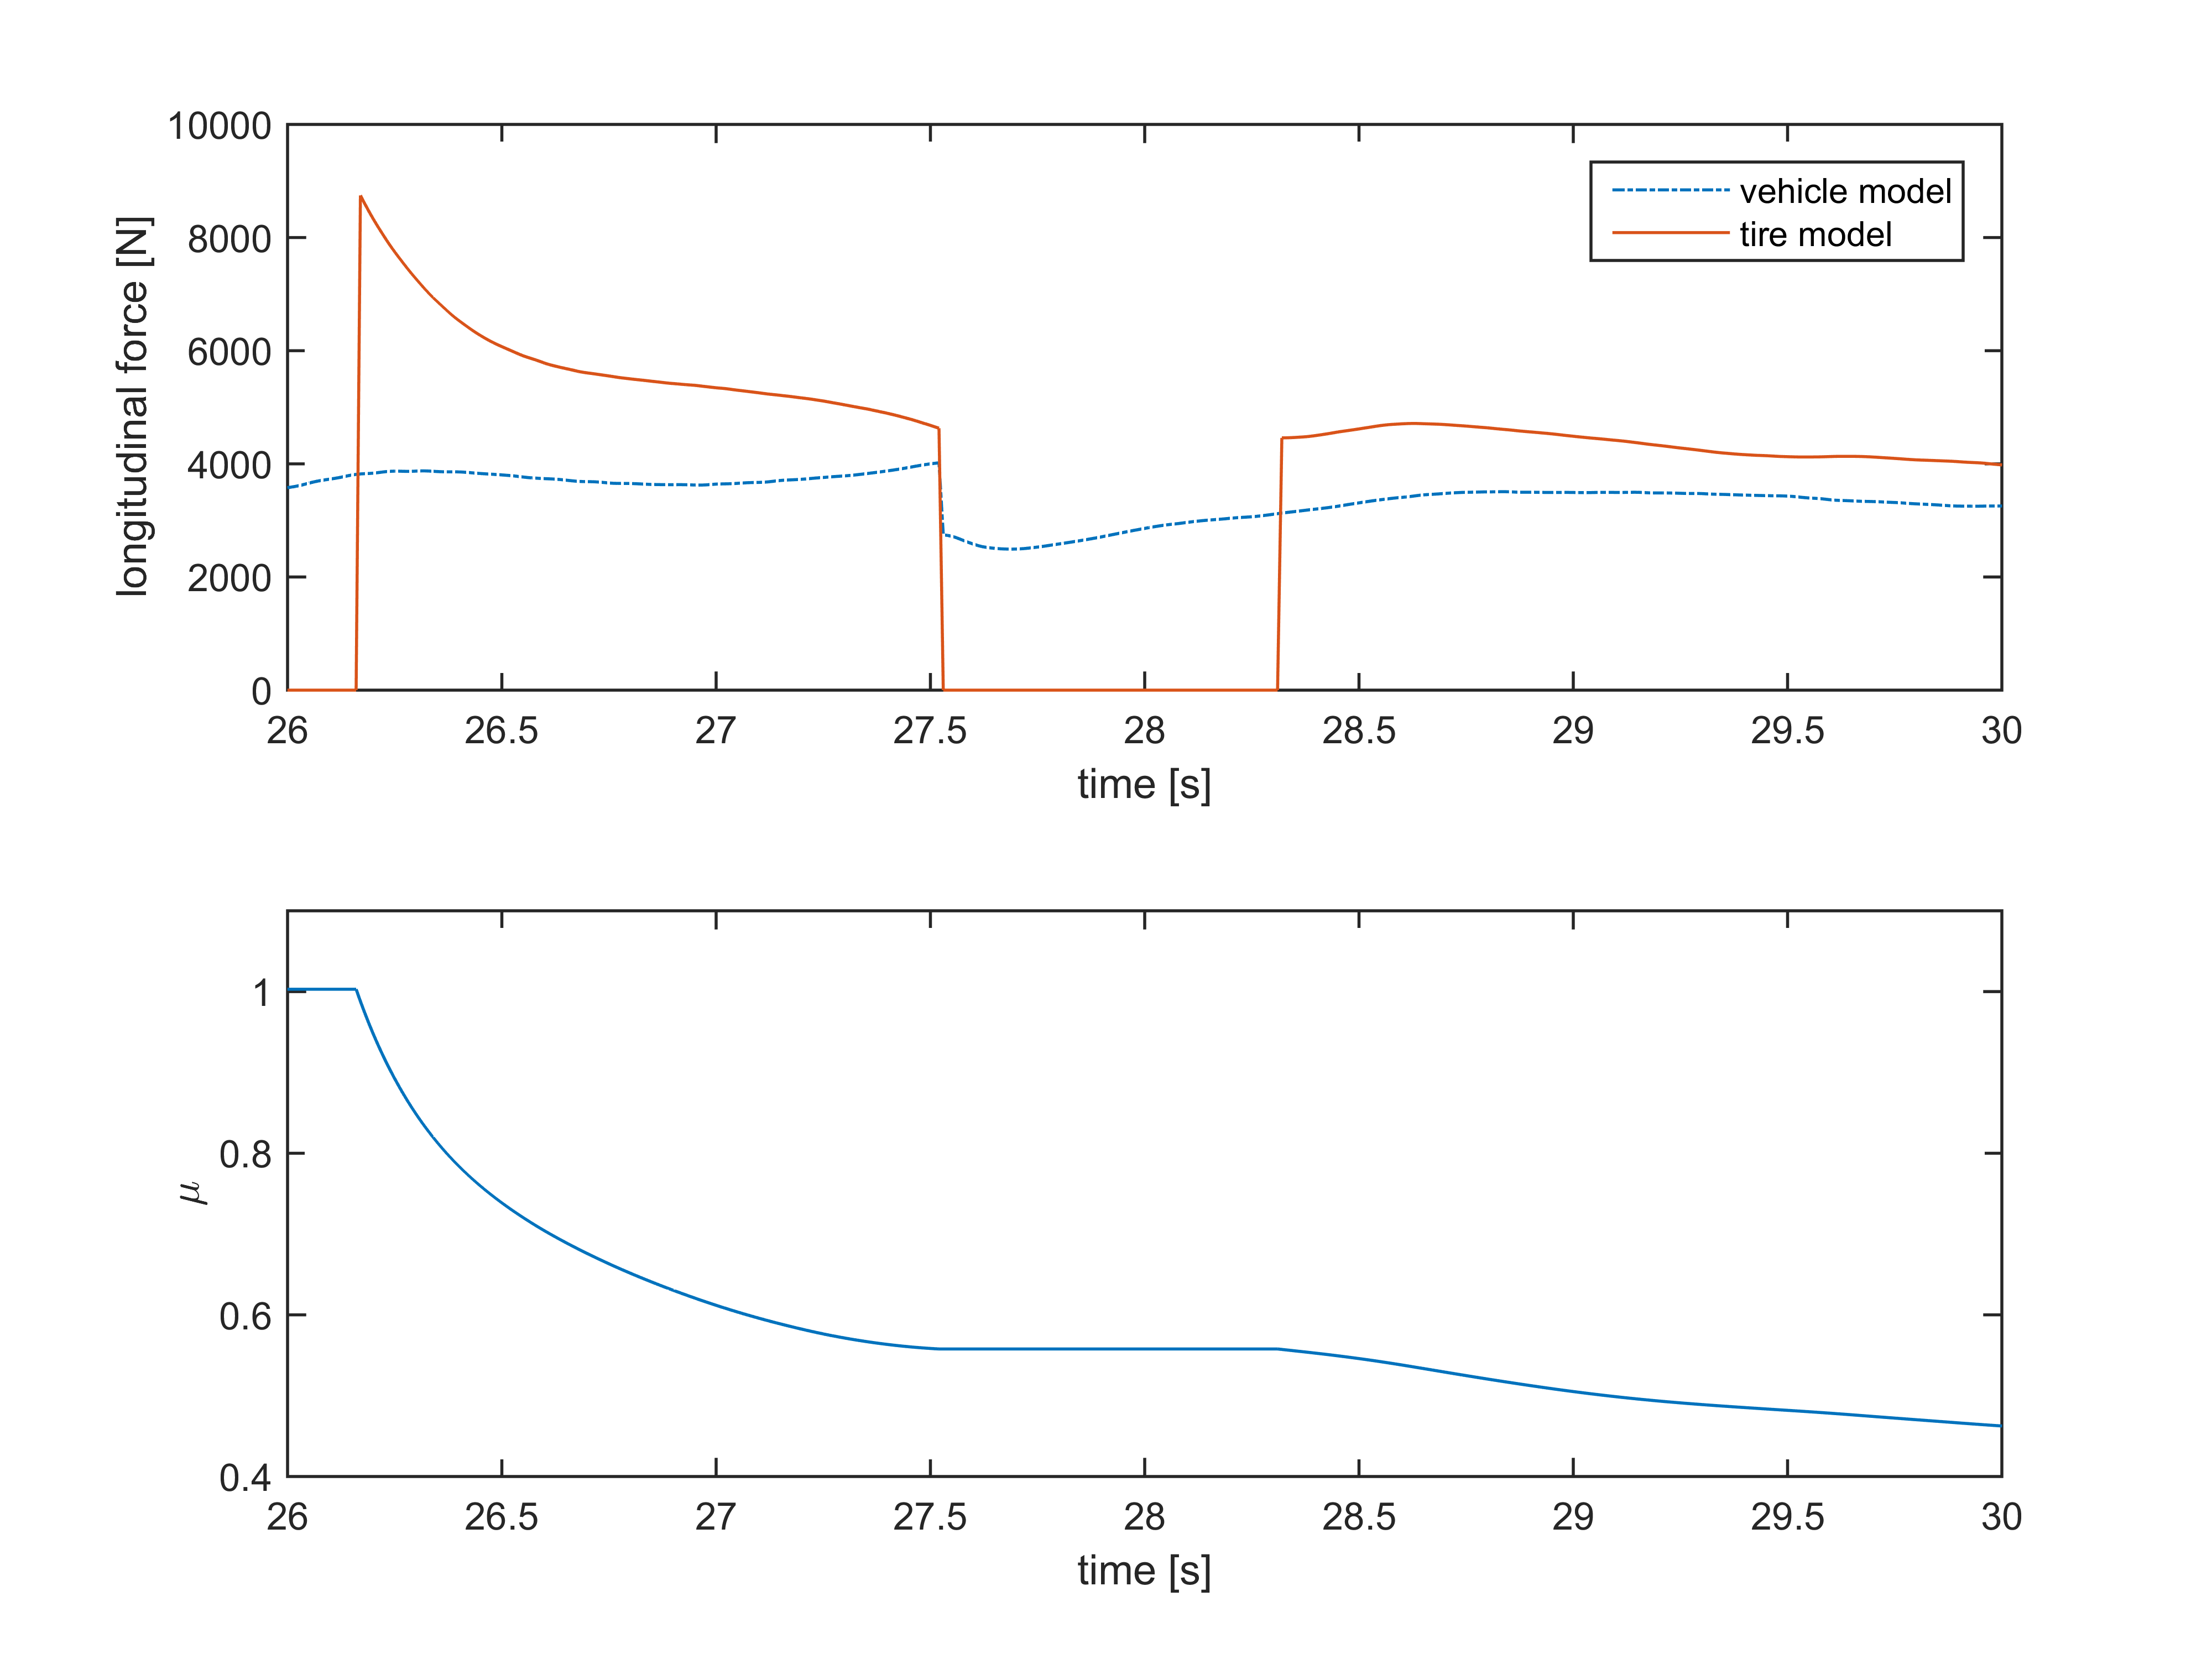
\includegraphics[width=1.0\textwidth]{Pictures/force_mue_comb2_zoom}
	\caption {Zoomed in picture of Figure \ref{force_mue_comb2}, showing how fast the new friction coefficient is found.}
	\label{force_mue_comb2_zoom}
\end{figure}

The normalized force per slip ratio for this combined sequence can be seen in Figure \ref{slip_kraft_comb2}. Note that this figure is is merely the two Figures \ref{slip_kraft_ljungby} and \ref{slip_kraft_is} merged together, with some erroneous result present around the times where the friction coefficient suddenly changes. The result clearly shows that a tire's stiffness varies for the two different surfaces.

\begin{figure}[h]
	\centering
	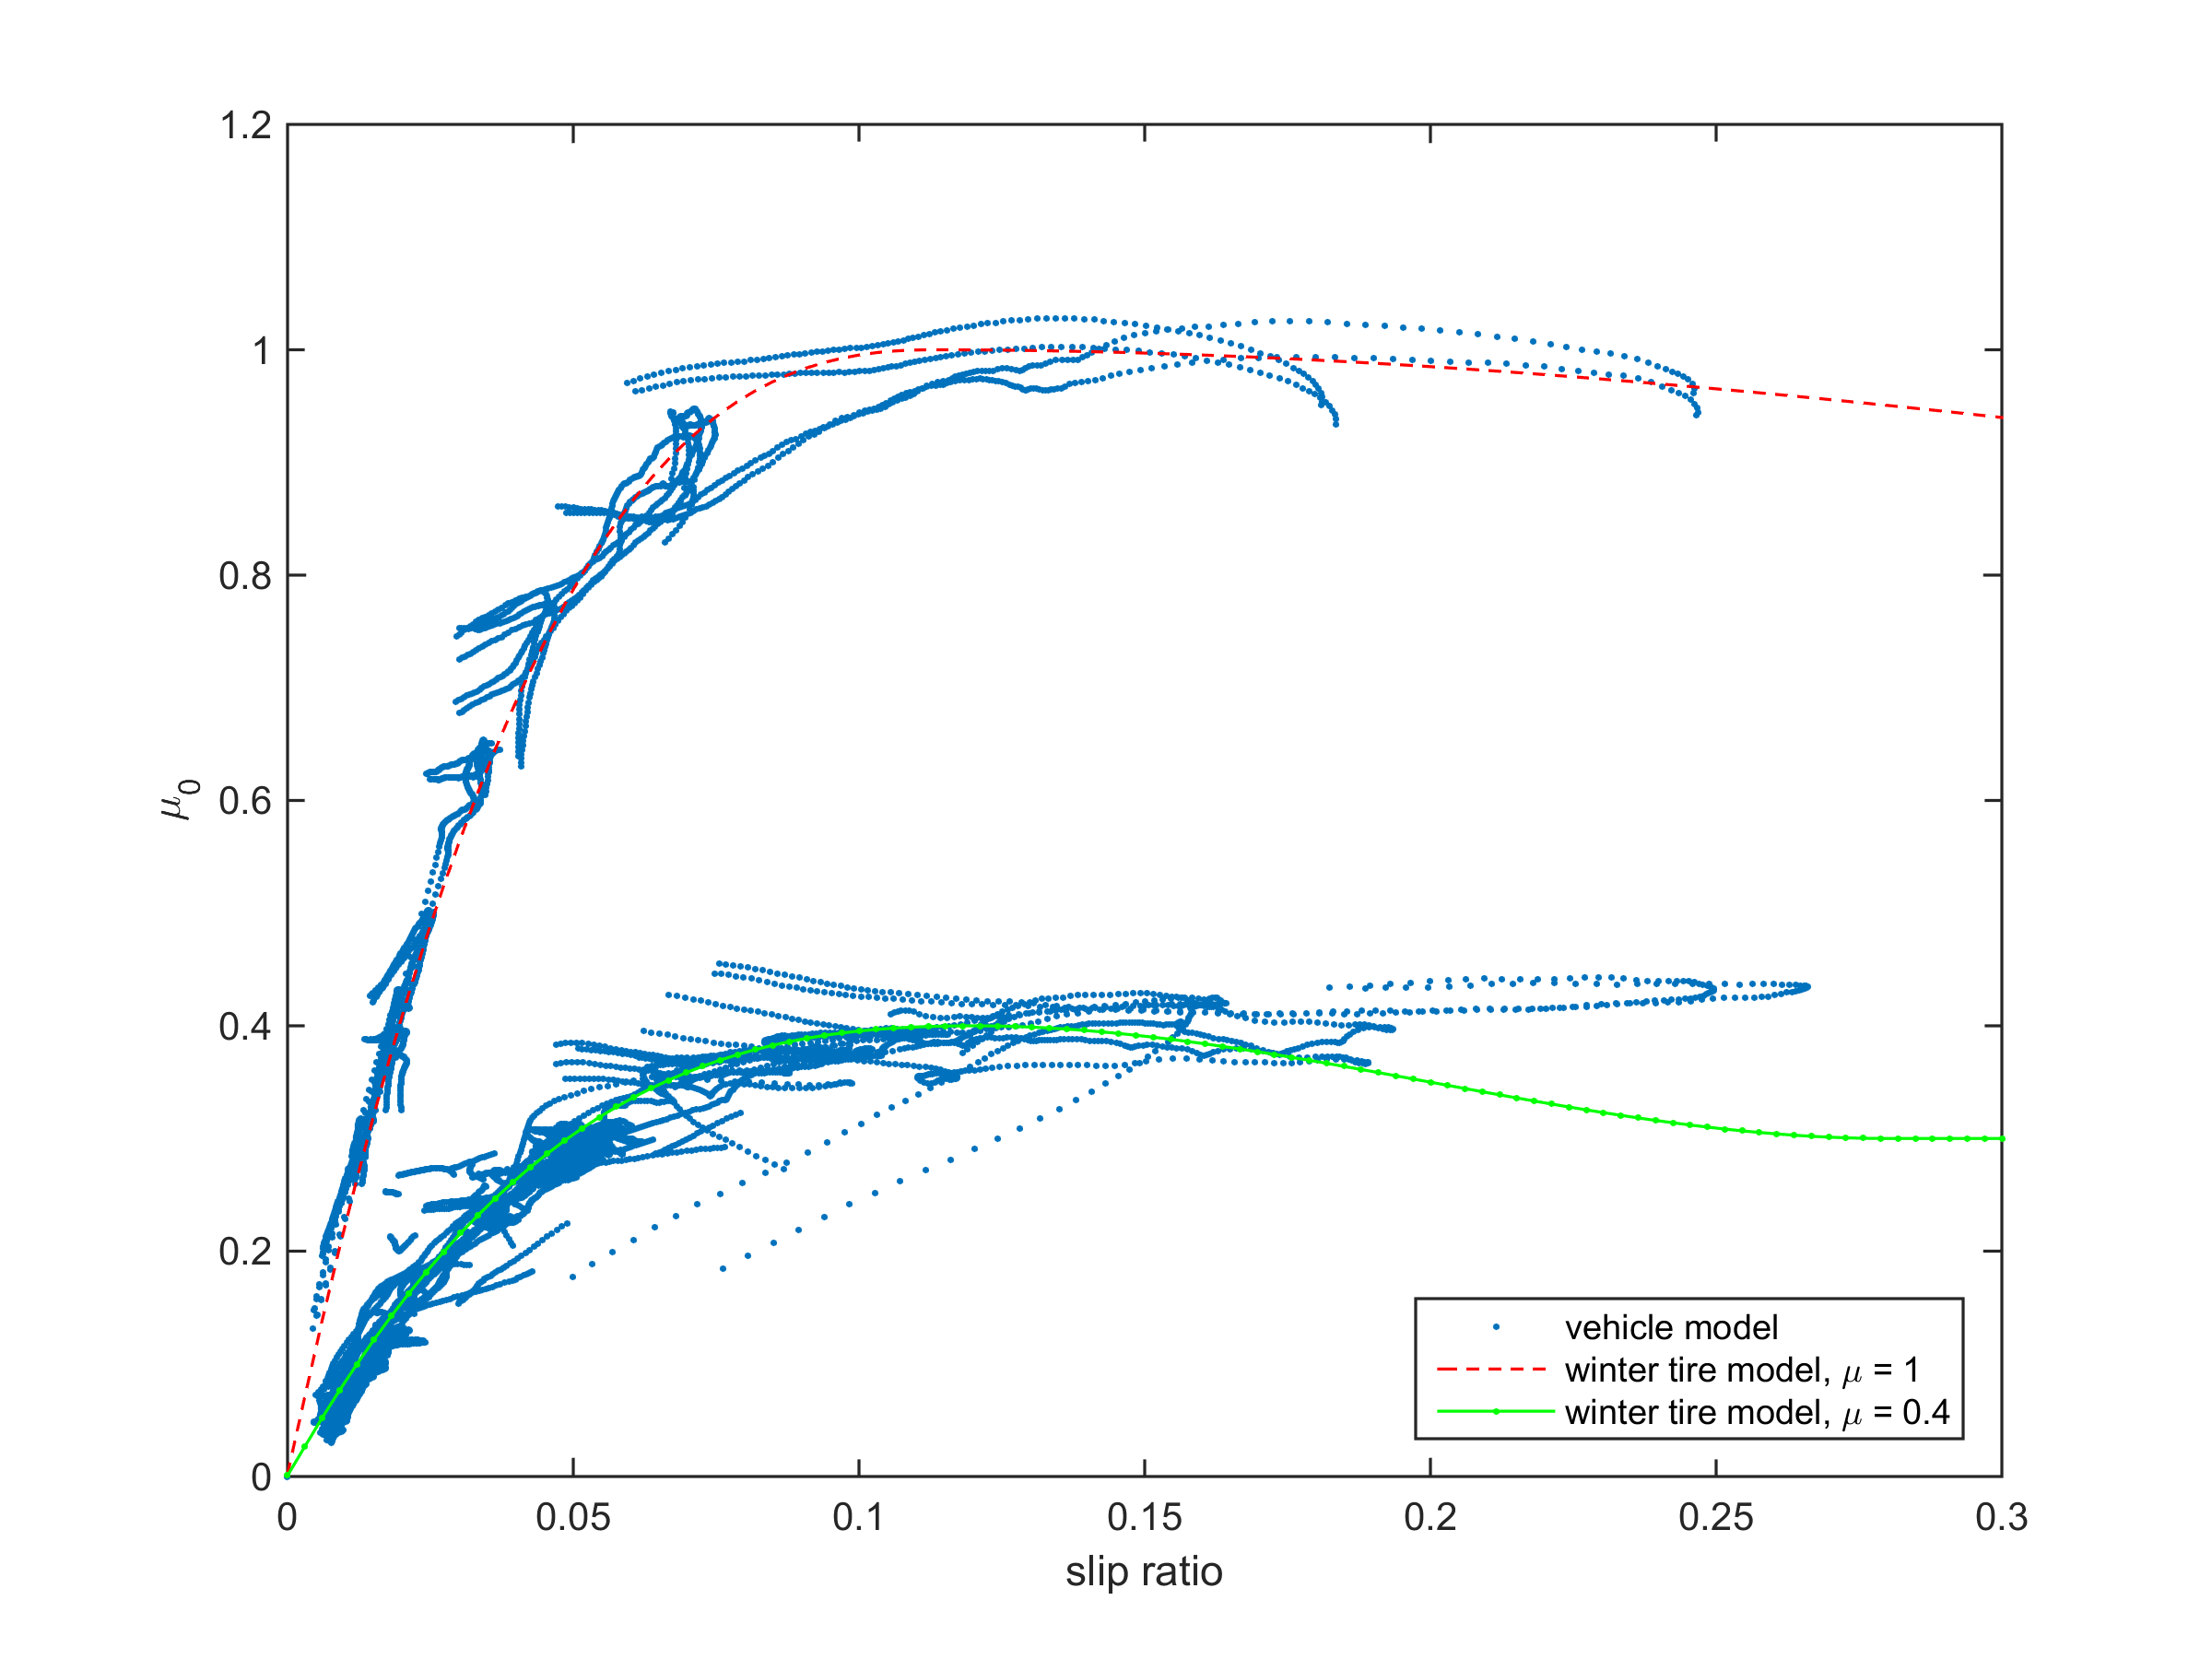
\includegraphics[width=1.0\textwidth]{Pictures/slip_kraft_comb2}
	\caption {Force per slip ratio for the combined driving sequence with both low- and high-$ \mu $.}
	\label{slip_kraft_comb2}
\end{figure}

\subsection{Summer tires on asphalt}


\subsection{Summer tires on wet asphalt}

\section{The used CAN signals}
Explain which signals are used throughout the report. Why are some not needed?.
